\documentclass[UTF8]{ctexart}
\usepackage{amsmath}
\usepackage{siunitx}
\usepackage{graphicx}
\usepackage{float}
\title{物理整理}
\author{kegalas}
\date{\today}

\begin{document}
    \maketitle
    \tableofcontents
    \newpage
    \section{速度增量法}
        适用于弹性碰撞。\\
        \indent 设小球1初速度为$v_{01}$质量为$m_1$,小球2初速度为$v_{02}$质量为$m_2$,($v_{01}>v_{02}$)求碰撞结束后小球1的速度$v_1$和小球2的速度$v_2$。
        \\
        \indent 可以看作小球1先减速,小球2先加速,一直到形变完成,此时两小球共速,速度为$v_{s}$。
        然后两小球恢复形变小球1减速,小球2加速,直到分开。
        经过推导得到小球1两次过程中速度变化量相同,记为$\Delta v_1$,小球2两次的变化量也相同,记为$\Delta v_2$。\\
        即为:
        \[v_{01}+\Delta v_1=v_s \quad v_s+\Delta v_1=v_1\]
        \[v_{02}+\Delta v_2=v_s \quad v_s+\Delta v_2=v_2\]
        所以有:
        \[v_{01}+v_1=2v_s\]
        \[v_{02}+v_2=2v_s\]
    \section{微元法}
        \begin{figure}[H]
            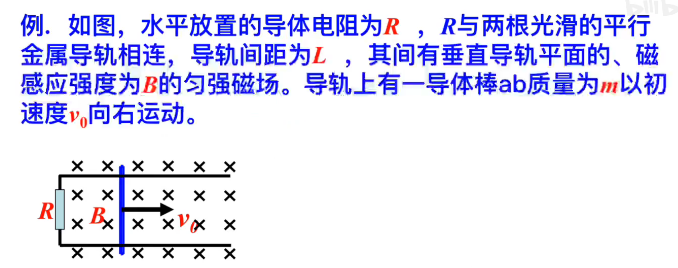
\includegraphics{2-1.png}
            \caption{例题1}
        \end{figure}
        我们要求出这个过程的总位移:
        \[-\frac{B^2 L^2 v}{R}=ma\]
        \[-\frac{B^2 L^2 v_i}{R}=m\frac{\Delta v_i}{\Delta t}\]
        \[-\frac{B^2 L^2 }{R}v_i\cdot \Delta t=m\Delta v_i\]
        \[-\frac{B^2 L^2 }{R}\Sigma v_i\cdot \Delta t=m\Sigma \Delta v_i\]
        \[-\frac{B^2 L^2 }{R}\Sigma \Delta x=m(0-v_0)\]
        \[\frac{B^2 L^2 }{R}x=m v_0\]
        \[x=\frac{m v_0 R}{B^2 L^2}\]
\end{document}